\title{Constrained Optimization with a Repeated Eigenvalue}
\subtitle{\SubTitleName}
\institute[]{\Course}
\author{\Instructor}
\maketitle   
   

\frame{\frametitle{Topics and Objectives}
\Emph{Topics} \\
%\TopicStatement
\begin{itemize}

    \item constrained optimization as an eigenvalue problem
    % \item distance and orthogonality constraints

\end{itemize}

\vspace{0.5cm}

\Emph{Learning Objectives}\\

%\LearningObjectiveStatement

\begin{itemize}

    \item apply eigenvalues and eigenvectors to solve a class of optimization problems that are subject to a distance constraint % and orthogonality constraints.
    
\end{itemize}
} 

\begin{frame}\frametitle{Example}

    Calculate the maximum and minimum values of $Q(\vec x) = \vec x^{\, T}A \vec x$, $\vec x \in \mathbb R^3$, subject to $||\vec x|| = 1$, and identify points where these values are obtained. 
    
    $$Q(\vec x) = x_1^2 + 2x_2x_3$$
\end{frame}
    
\begin{frame}\frametitle{Example Solution}
    
    For $Q(\vec x) = x_1^2 + 2x_2x_3$, we have
    \begin{align*}
        Q &= \vec x \, ^T A\vec x,\quad A = \spalignmat{1 0 0;0 0 1;0 1 0} 
    \end{align*}
    \pause By inspection, $A$ has eigenvalues $\pm 1$ (don't forget that an eigenvalue, $\lambda$, is a number that makes $A - \lambda I$ singular). For $\lambda = 1$, 
    \pause 
    \begin{align*}
        A-I = \spalignmat{0 0 0;0 -1 1;0 1 -1} \Rightarrow \vec v_1 = \spalignmat{1;0;0}, \vec v_2 = \frac{1}{\sqrt2}\spalignmat{0;1;1}
    \end{align*}
\end{frame}
    
\begin{frame}\frametitle{Example Solution}    
    Because $A$ is symmetric, the eigenvector for eigenvalue $\lambda = -1$ must be orthogonal to $\vec v_1$ and $\vec v_2$. \pause So by inspection $$\vec v_3 = \frac{1}{\sqrt{2}}\spalignmat{0;1;-1}$$
    \pause Therefore, the minimum value of $Q$ is $-1$, and is obtained at $\pm \vec v_3$. \pause The maximum value of $Q$ is $+1$, which is obtained at any unit vector in the span of $\vec v_1$ and $\vec v_2$. 
\end{frame}


\begin{frame}\frametitle{Example Solution}    

    The image below is the unit sphere whose surface is colored according to the quadratic from the previous example. Notice the agreement between our solution and the image. 

    \begin{center}
        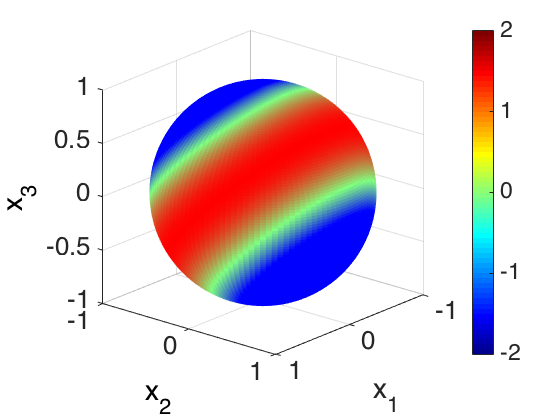
\includegraphics[width=0.5\textwidth]{Chapter7/images/sphere73example2.png} 
    \end{center}

\end{frame}

\frame{\frametitle{Summary}

    \SummaryLine \vspace{4pt}
    \begin{itemize}\setlength{\itemsep}{8pt}

        \item constrained optimization problems of the form: identify the maximum/minimum values (and where they are located) of $$Q(\vec x) = \vec x^{\, T}A \vec x$$ subject to $$||\vec x|| = 1$$
        \item we saw that the maximum/minimum values are given by eigenvalues of $A$
        \item we saw that the locations where these extreme values are given by unit eigenvectors of $A$

    \end{itemize}
    
    \vspace{6pt}

    \pause
}



